\documentclass[10pt,twocolumn]{article}
\usepackage[a4paper,margin=0.68in]{geometry}
\usepackage{graphicx,booktabs,amsmath,microtype,xcolor,hyperref,natbib}
\usepackage[T1]{fontenc}
\hypersetup{colorlinks=true,allcolors=blue!55!black}
\newcommand{\TestCases}{35}
\newcommand{\FullACC}{0.347}
\newcommand{\EqualACC}{0.307}
\newcommand{\SelectedACC}{0.296}
\newcommand{\FullRMSE}{4.989}
\newcommand{\EqualRMSE}{5.174}
\newcommand{\FullBias}{-0.303}
\newcommand{\EqualBias}{-0.428}
\newcommand{\FullEqualEffect}{0.040}
\newcommand{\FullEqualLow}{0.011}
\newcommand{\FullEqualHigh}{0.070}
\newcommand{\FullSelectedEffect}{0.052}
\newcommand{\FullSelectedLow}{-0.002}
\newcommand{\FullSelectedHigh}{0.093}
\newcommand{\ForecastLocationEffect}{0.238}
\newcommand{\ForecastLocationLow}{0.209}
\newcommand{\ForecastLocationHigh}{0.266}


\title{Lightweight Post-processing of Multi-model Subseasonal Rainfall Forecasts over India: A Leakage-Safe 2025 Benchmark}
\author{Anonymous authors}
\date{}

\begin{document}
\maketitle

\begin{abstract}
Reliable weekly rainfall guidance at subseasonal leads can support climate
adaptation decisions, yet heterogeneous model calendars, grids, climatologies,
and test reuse make regional comparisons fragile. We construct a valid-date-
aligned benchmark of seven physics, data-driven, and hybrid systems over India
for JJAS initializations and lead Weeks 1--6. All forecasts and India
Meteorological Department (IMD) observations use one 1.5-degree grid, one
1991--2019 IMD climatology, and identical fractional-area support. We freeze
training (2020--2023), validation (2024), metrics, hyperparameters, and
ablations before opening \,\TestCases{} common 2025 initializations. An
XGBoost adaptation of PiggyCast raises mean case-level spatial ACC from
\EqualACC{} for equal weighting to \FullACC{} (paired difference
\FullEqualEffect{}, 95\% moving-block interval [\FullEqualLow{},
\FullEqualHigh{}]) and reduces RMSE from \EqualRMSE{} to \FullRMSE{} mm
day$^{-1}$. Forecast-conditioned features substantially outperform a
location/calendar-only ablation. However, the ACC difference from the
validation-selected individual system is \FullSelectedEffect{}
[\FullSelectedLow{}, \FullSelectedHigh{}], failing our predeclared headline
gate; ACC also deteriorates relative to equal weighting at Weeks 5--6 and in
east/northeast India. Lightweight mixing is therefore promising but not
uniformly superior. The case-level metrics, uncertainty intervals, frozen
protocol, trained models, and hashes make this bounded result fully auditable.
\end{abstract}

\section{Introduction}

The two-to-six-week range bridges weather prediction and seasonal outlooks,
with potential value for water management, agriculture, heat and flood
preparedness, and other adaptation decisions. The WWRP/WCRP S2S database made
multi-centre forecast comparison possible \citep{vitart2017s2s}, while recent
AI systems such as FuXi-S2S \citep{chen2024fuxi}, NeuralGCM
\citep{kochkov2024neuralgcm}, and DLESyM \citep{cresswellclay2024dlesym}
expand the set of forecast architectures. Diversity alone does not guarantee
that a multi-model mean is optimal, particularly for monsoon rainfall and
spatially heterogeneous model biases.

We ask a deliberately narrow question: can data-efficient post-processing
improve weekly India rainfall forecasts without retraining the underlying
systems? Our contributions are: (i) a seven-system benchmark with exact
initialization and valid-date alignment; (ii) a regional adaptation of
PiggyCast \citep{kimani2025piggycast} using forecast-conditioned gradient-
boosted trees; and (iii) a confirmatory 2025 evaluation with predeclared claim
gates and paired uncertainty. The outcome is useful precisely because it is
not uniformly positive: adaptive mixing clears the equal-weight and feature-
ablation gates but not the stronger validation-selected-model gate.

\begin{figure*}[t]
  \centering
  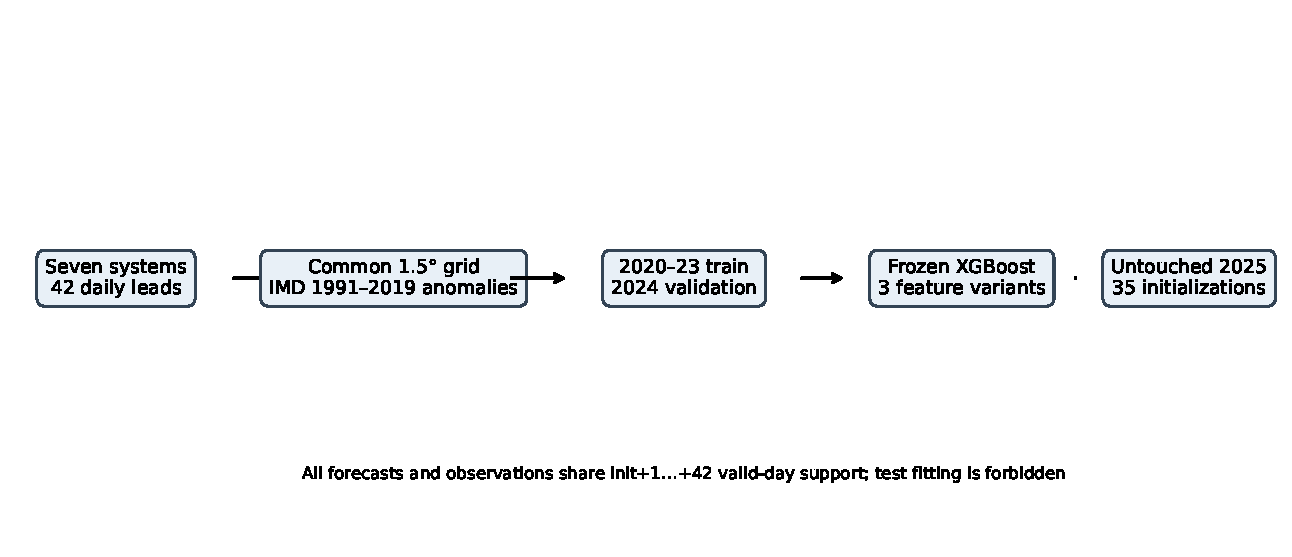
\includegraphics[width=0.96\textwidth]{../artifacts/confirmatory_2025/figures/pipeline.pdf}
  \caption{Leakage-safe workflow. The 2025 forecast values were opened only
  after the complete protocol and metadata-only coverage preflight were frozen.}
  \label{fig:pipeline}
\end{figure*}

\section{Data and harmonization}

\paragraph{Forecasts.}
We evaluate CMA, DLESyM v0, ECMWF, FuXi-S2S, NCEP, NeuralGCM, and UKMO weekly
ensemble-mean precipitation. Table~\ref{tab:inventory} summarizes the products.
Each case has 42 complete daily rates. Lead Week 1 averages intervals ending
initialization+1 through +7 days; Week 6 averages +36 through +42. We retain
small negative finite precipitation increments produced by differencing rather
than silently clipping them. Five systems use immutable standardized 2025
stores; DLESyM and NeuralGCM use native 2025 files whose units, coordinates,
and period endpoints match the same archive contract.

\begin{table}[t]
\centering\small
\caption{Forecast inventory. The 2024 common validation intersection contains
30 cases; 2020--2023 and 2025 contain 35 per year.}
\label{tab:inventory}
\resizebox{\columnwidth}{!}{\begin{tabular}{llrrr}
\toprule
System & Type & Members & 2020--23 cases/year & 2025 cases \\
\midrule
CMA operational & physics & 4 & 35 & 35 \\
DLESyM v0 & AI Earth system & 1 & 35 & 35 \\
ECMWF operational & physics & 51 or 101 & 35 & 35 \\
FuXi-S2S & AI subseasonal & 50 & 35 & 35 \\
NCEP operational & physics & 16 & 35 & 35 \\
NeuralGCM & hybrid AI--physics & 10 & 35 & 35 \\
UKMO operational & physics & 4 & 35 & 35 \\
\bottomrule
\end{tabular}
}
\end{table}

\paragraph{Truth, grid, and anomalies.}
IMD gauge-based daily rainfall \citep{pai2014imd} is conservatively aggregated
to a 27$\times$27, 1.5-degree grid spanning 0--39$^\circ$N and
60--99$^\circ$E. Grid-cell weights multiply spherical area, fractional India
or regional overlap, and IMD observation fraction. A fixed 31-day-window IMD
1991--2019 normal is averaged over each forecast's exact seven valid dates and
subtracted from both forecast and observation. No model-specific climatology
enters any ACC calculation.

\paragraph{Splits and coverage.}
We train with 140 JJAS cases from 2020--2023, use the 30-case common 2024
intersection for all selection, and test once on 35 common 2025 cases. The five
missing 2024 initializations are June 6, 10, 13, 17 and August 5. Later lead
windows may verify after September because season membership is defined by the
initialization date.

\section{Methods}

\paragraph{Baselines.}
We retain all seven individual ensemble means. The equal-weight baseline is the
arithmetic multi-model mean. A validation-weighted mean uses non-negative,
per-week inverse 2024 RMSE weights. A validation-selected baseline takes the
lowest-2024-RMSE individual model separately at each lead: FuXi-S2S at Week 1
and ECMWF at Weeks 2--6.

\paragraph{Adaptive mixing.}
Following PiggyCast, we fit one XGBoost regressor \citep{chen2016xgboost} per
lead week. Forecast-only inputs comprise seven forecast anomalies and six real
ensemble-spread fields (DLESyM is deterministic). The full variant adds
latitude, longitude, and sine/cosine of verification-midpoint day of year. A
location/calendar-only ablation removes all forecast information. Hyperparameters
are fixed at maximum depth 4, learning rate 0.03, subsample 0.8, column
subsample 0.9, and at most 600 trees. Early stopping on 2024 chooses the tree
count; a fresh estimator with that count is refit on 2020--2024, then applied
to 2025. Area weights are used during fitting and validation.

\paragraph{Verification and uncertainty.}
The primary score is case-level area-weighted spatial anomaly correlation
(ACC), averaged equally across initialization--week cases. Secondary metrics
are RMSE, MAE, signed bias, and wet-area fraction error at 1 mm day$^{-1}$.
We report paired percentile intervals from 2,000 circular moving-block draws
over ordered initialization dates, retaining all six leads together. The
primary block length is four initializations; lengths 2 and 8 are sensitivities.
Intervals are descriptive effect intervals rather than $p$-values.

\section{Confirmatory 2025 results}

\subsection{Overall and lead-dependent skill}

Full PiggyCast attains ACC \FullACC{}, RMSE \FullRMSE{}, MAE 3.603, and bias
\FullBias{} mm day$^{-1}$, compared with equal-weight ACC \EqualACC{}, RMSE
\EqualRMSE{}, MAE 3.716, and bias \EqualBias{}. The paired ACC gain over equal
weight is \FullEqualEffect{} [\FullEqualLow{}, \FullEqualHigh{}], and its RMSE
difference is -0.186 [-0.290, -0.096] mm day$^{-1}$. Inverse-validation-RMSE
weighting yields a smaller ACC improvement, 0.313 versus 0.307.

Figure~\ref{fig:lead} shows strong lead dependence. Full PiggyCast improves ACC
over equal weighting at Weeks 1--4 (by 0.057, 0.064, 0.070, and 0.099), is
nearly tied at Week 5 (-0.001), and is worse at Week 6 (-0.047). Its RMSE is
lower at every lead. This divergence reinforces the need to report both
pattern and amplitude metrics.

\begin{figure*}[t]
  \centering
  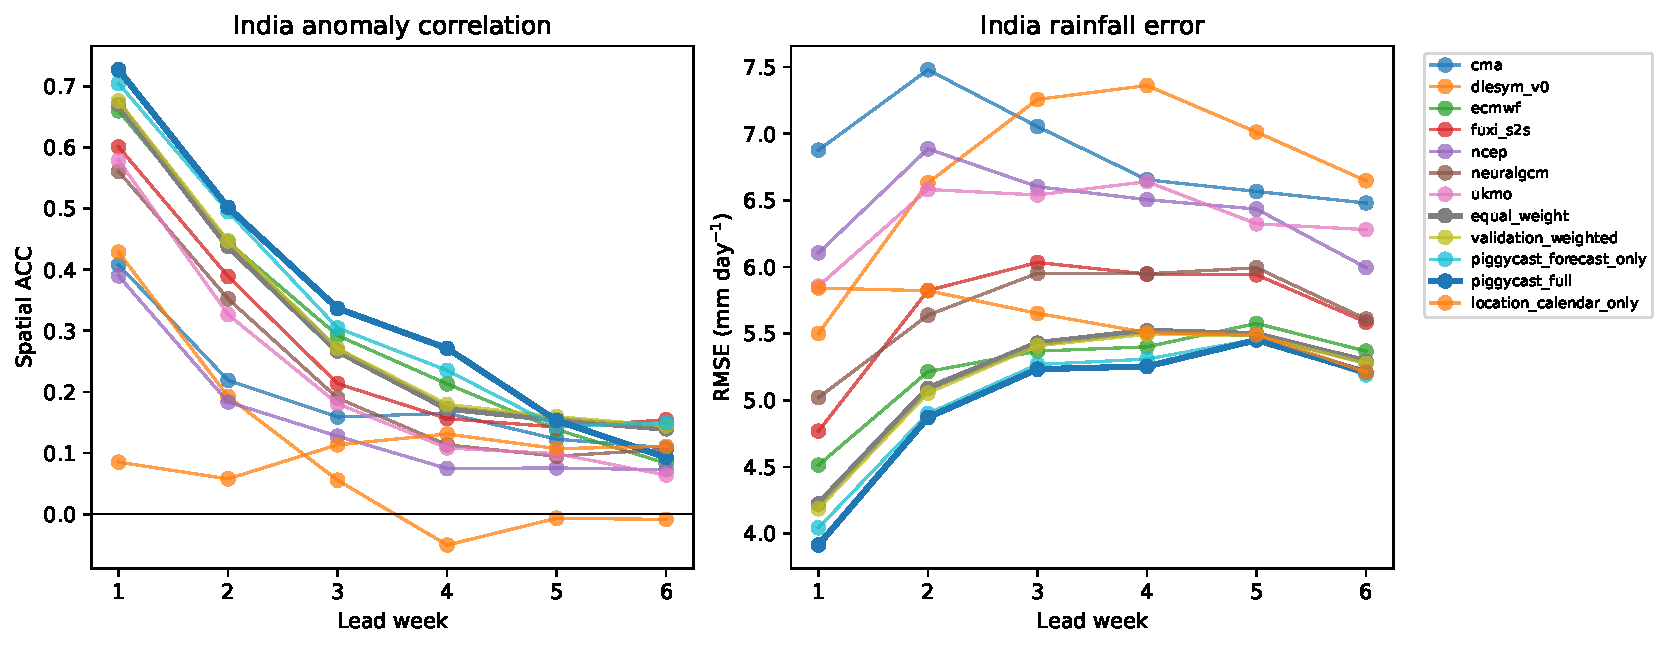
\includegraphics[width=0.95\textwidth]{../artifacts/confirmatory_2025/figures/skill_by_lead.pdf}
  \caption{India-area-weighted case-mean spatial ACC and RMSE by lead.}
  \label{fig:lead}
\end{figure*}

\begin{table*}[t]
\centering\small
\caption{Overall 2025 scores across 35 initializations and six lead weeks.
Wet-area error is forecast minus observed weighted wet fraction.}
\label{tab:overall}
\begin{tabular}{lrrrrr}
\toprule
Method & ACC $\uparrow$ & RMSE $\downarrow$ & MAE $\downarrow$ & Bias & Wet-area error \\
\midrule
piggycast\_full & 0.347 & 4.989 & 3.603 & -0.303 & 0.113 \\
piggycast\_forecast\_only & 0.339 & 5.028 & 3.626 & -0.288 & 0.117 \\
validation\_weighted & 0.313 & 5.150 & 3.700 & -0.397 & 0.114 \\
equal\_weight & 0.307 & 5.174 & 3.715 & -0.428 & 0.114 \\
ecmwf & 0.305 & 5.240 & 3.822 & 0.253 & 0.107 \\
validation\_selected\_model & 0.296 & 5.283 & 3.845 & 0.157 & 0.097 \\
fuxi\_s2s & 0.276 & 5.683 & 4.014 & -0.363 & 0.047 \\
neuralgcm & 0.236 & 5.694 & 4.094 & -0.429 & 0.099 \\
ukmo & 0.226 & 6.370 & 4.522 & 0.328 & 0.044 \\
cma & 0.197 & 6.852 & 4.839 & -0.364 & 0.052 \\
ncep & 0.154 & 6.421 & 4.538 & -1.471 & -0.013 \\
dlesym\_v0 & 0.102 & 6.735 & 4.815 & -0.950 & 0.010 \\
location\_calendar\_only & 0.101 & 5.587 & 4.091 & -0.402 & 0.144 \\
\bottomrule
\end{tabular}

\end{table*}

\subsection{Gates, ablations, and regional behavior}

The forecast-only variant exceeds the location/calendar-only ablation by
\ForecastLocationEffect{} ACC [\ForecastLocationLow{},
\ForecastLocationHigh{}], showing that the gain cannot be attributed to a
learned seasonal spatial normal alone. Adding calendar/location features to
the forecast-only model raises overall ACC from 0.339 to 0.347 and reduces
RMSE from 5.028 to 4.989.

The stronger comparison is inconclusive. Full PiggyCast exceeds the
validation-selected model in mean ACC by \FullSelectedEffect{}, but its
interval [\FullSelectedLow{}, \FullSelectedHigh{}] overlaps zero. Our frozen
gate therefore prohibits the headline claim that adaptive mixing is robustly
better than the selected individual system, despite favorable RMSE and bias
guards.

Regional mean ACC differences relative to equal weighting are +0.128 in
northwest India, +0.060 in the south peninsula, +0.011 in central India, and
-0.097 in east/northeast India. Figure~\ref{fig:paired} displays paired overall
and regional intervals. The three-of-four positive-region gate passes, but the
east/northeast failure precludes language implying geographically uniform
benefit.

\begin{table}[t]
\centering\small
\caption{Predeclared paired ACC comparisons with 95\% moving-block intervals.}
\label{tab:ablations}
\resizebox{\columnwidth}{!}{\begin{tabular}{lrrr}
\toprule
Paired ACC comparison & Mean & 2.5th pct. & 97.5th pct. \\
\midrule
Full $-$ equal weight & 0.040 & 0.011 & 0.070 \\
Full $-$ validation-selected & 0.052 & -0.002 & 0.093 \\
Forecast-only $-$ location/calendar & 0.238 & 0.209 & 0.266 \\
\bottomrule
\end{tabular}
}
\end{table}

\begin{figure*}[t]
  \centering
  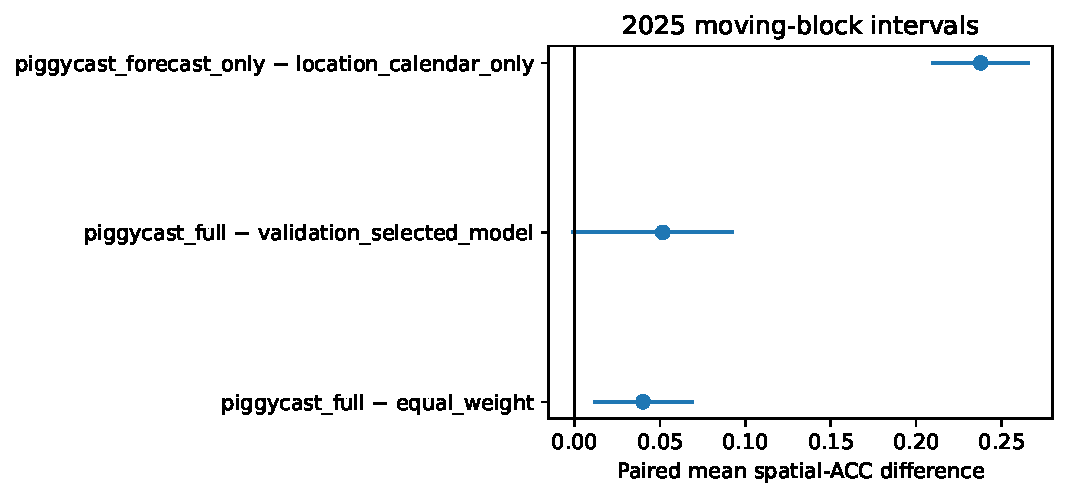
\includegraphics[width=0.48\textwidth]{../artifacts/confirmatory_2025/figures/paired_acc.pdf}
  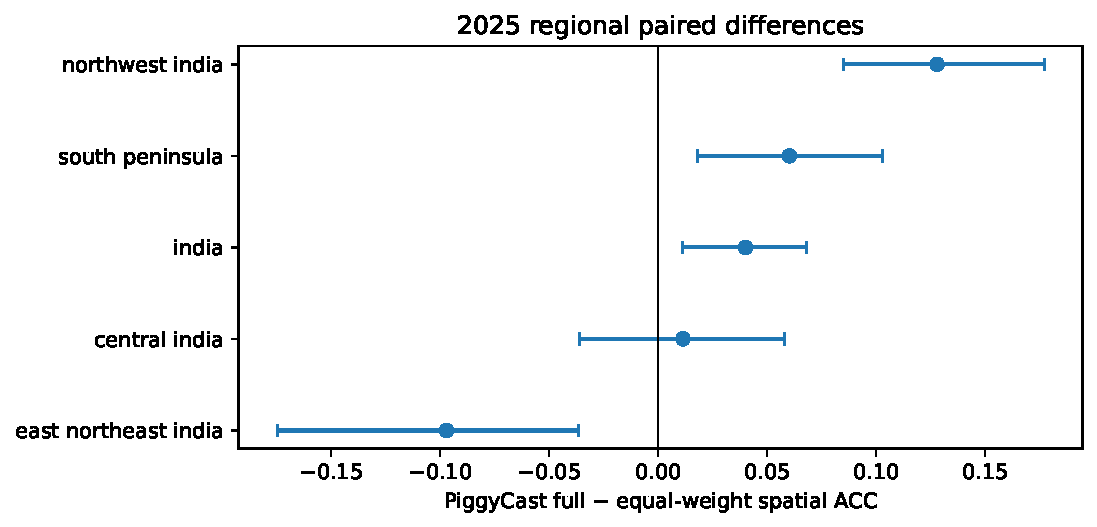
\includegraphics[width=0.48\textwidth]{../artifacts/confirmatory_2025/figures/regional_acc.pdf}
  \caption{Paired 2025 ACC differences. Bars are 95\% circular moving-block
  percentile intervals over initialization dates; all six leads remain grouped.}
  \label{fig:paired}
\end{figure*}

\section{Discussion}

The results support a bounded operational proposition: a compact post-processor
can extract complementary information from heterogeneous forecast systems and
outperform an uncalibrated equal-weight mean without changing the underlying
models. The forecast-only ablation provides direct evidence that the method
uses forecast state, while the lower RMSE and less negative bias argue against
an ACC-only artifact.

The failed selected-model gate is equally important. First, 35 test
initializations give limited precision under serial dependence. The comparison
changes with bootstrap block length: its lower endpoint is +0.009 for length 2
but -0.002 at lengths 4 and 8, whereas the equal-weight comparison remains
positive at all three lengths. Second, selected tree counts collapse from
hundreds at Weeks 1--3 to 8--12 at Weeks 5--6, consistent with weak conditional
signal at long leads. Third, geographic transfer is uneven, with a clear
east/northeast loss. A production system should therefore retain per-lead and
regional guardrails rather than deploying one national aggregate decision.

This study evaluates deterministic ensemble means and does not assess
probabilistic calibration, extremes, onset timing, or decision value. Model
versions and operational ensemble sizes differ, and the 2024 validation archive
has a five-date gap. The fixed IMD normal avoids cross-method climatology
leakage but a single 1991--2019 baseline cannot resolve nonstationarity. Finally,
the compact FuXi neural correction planned as a complementary method is absent:
its existing frozen evaluator uses initialization+0--6 day labels, inconsistent
with the benchmark's +1--7 period endpoints. We report this as a negative
workflow finding rather than compare misaligned scores.

\section{Conclusion}

We provide a reproducible seven-system India S2S rainfall benchmark and a
leakage-safe test of lightweight adaptive mixing. PiggyCast improves overall
2025 ACC and RMSE relative to equal weighting and clearly outperforms a
location/calendar-only ablation. It does not clear the predeclared uncertainty
gate against the validation-selected individual system and loses ACC at the
longest leads and in east/northeast India. The appropriate conclusion is not
that post-processing is uniformly best, but that forecast-conditioned mixing
has measurable, region- and lead-dependent value that warrants broader testing.

\section*{Reproducibility statement}

The supplementary bundle contains the frozen JSON protocol, exact coverage,
case-level metrics, aggregate tables, paired intervals, bootstrap sensitivity,
18 serialized XGBoost models, figures, source and artifact hashes, and an audit
report. The audit independently regenerates every aggregate score from the
case table. No 2025 fitting, threshold selection, feature selection, or retry
selection is performed.

\bibliographystyle{plainnat}
\bibliography{references}

\appendix
\section{Supplementary material}

All reported appendix scores use IMD as the observational reference and the
same dates, grid, anomaly normal, and fractional-area support as the main
paper. No IMERG or temperature result is included in the current claims.

\subsection{Forecast inventory and coverage}

\begin{table*}[h]
\centering\small
\caption{Forecast cohort. The 2024 common intersection contains 30 cases;
2020--2023 and 2025 contain 35 per year. Operational ensemble size changes
where shown do not alter the ensemble-mean evaluation contract.}
\label{tab:inventory}
\resizebox{0.78\textwidth}{!}{\begin{tabular}{llrrr}
\toprule
System & Type & Members & 2020--23 cases/year & 2025 cases \\
\midrule
CMA operational & physics & 4 & 35 & 35 \\
DLESyM v0 & AI Earth system & 1 & 35 & 35 \\
ECMWF operational & physics & 51 or 101 & 35 & 35 \\
FuXi-S2S & AI subseasonal & 50 & 35 & 35 \\
NCEP operational & physics & 16 & 35 & 35 \\
NeuralGCM & hybrid AI--physics & 10 & 35 & 35 \\
UKMO operational & physics & 4 & 35 & 35 \\
\bottomrule
\end{tabular}
}
\end{table*}

The five missing 2024 common initializations are June 6, 10, 13, 17, and
August 5. Exact ISO dates are stored in \texttt{coverage.csv}; per-system
availability, coordinates, units, and source metadata hashes are stored in
\texttt{preflight/coverage\_preflight.csv} and
\texttt{preflight/preflight.json}. The metadata-only coverage preflight
records \texttt{forecast\_values\_read=false}. DLESyM and NeuralGCM 2025 files
enter through native-file adapters after the same coordinate, unit, and
42-period completeness checks as the standardized stores.

\subsection{All systems and all lead weeks}

\begin{table*}[h]
\centering\scriptsize
\caption{Complete 2025 national score table. RMSE, MAE, and bias are in mm
day$^{-1}$; wet-area error is forecast minus observed weighted fraction at
1 mm day$^{-1}$. Negative support is the area-weighted fraction of evaluated
support below zero under the no-clipping policy.}
\label{tab:all-methods}
\resizebox{\textwidth}{!}{\begin{tabular}{lrrrrrr}
\toprule
Method & ACC $\uparrow$ & RMSE $\downarrow$ & MAE $\downarrow$ & Bias & Wet-area error & Negative support (\%) \\
\midrule
PiggyCast, full & 0.347 & 4.989 & 3.603 & -0.303 & 0.113 & 0.52 \\
PiggyCast, forecast only & 0.339 & 5.028 & 3.626 & -0.288 & 0.117 & 0.16 \\
Validation-weighted mean & 0.313 & 5.150 & 3.700 & -0.397 & 0.114 & 0.00 \\
Equal-weight mean & 0.307 & 5.174 & 3.715 & -0.428 & 0.114 & 0.00 \\
ECMWF & 0.305 & 5.240 & 3.822 & 0.253 & 0.107 & 0.00 \\
Per-lead 2024-RMSE-selected & 0.296 & 5.283 & 3.845 & 0.157 & 0.097 & 0.00 \\
FuXi-S2S & 0.276 & 5.683 & 4.014 & -0.363 & 0.047 & 0.00 \\
NeuralGCM & 0.236 & 5.694 & 4.094 & -0.429 & 0.099 & 0.00 \\
UKMO & 0.226 & 6.370 & 4.522 & 0.328 & 0.044 & 0.00 \\
CMA & 0.197 & 6.852 & 4.839 & -0.364 & 0.052 & 0.06 \\
NCEP & 0.154 & 6.421 & 4.538 & -1.471 & -0.013 & 0.02 \\
DLESyM v0 & 0.102 & 6.735 & 4.815 & -0.950 & 0.010 & 0.00 \\
Location/calendar only & 0.101 & 5.587 & 4.091 & -0.402 & 0.144 & 0.06 \\
\bottomrule
\end{tabular}
}
\end{table*}

\begin{figure*}[h]
  \centering
  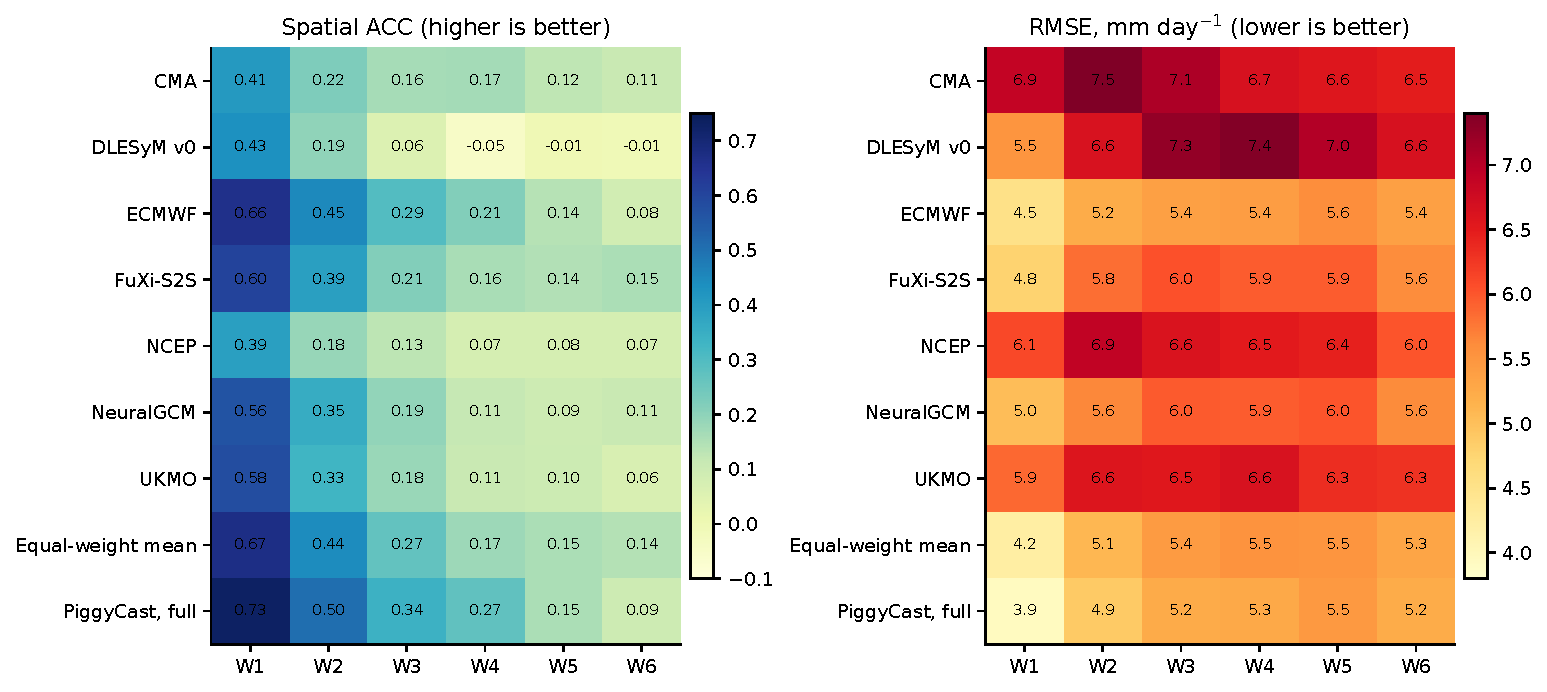
\includegraphics[width=\textwidth]{figures/appendix_all_models_imd.pdf}
  \caption{IMD-referenced 2025 national comparison for every base system,
  equal weighting, and full PiggyCast at Weeks 1--6. The defensible pattern is
  rapid, heterogeneous skill decay rather than a blanket statement that the
  systems are unskillful: several Week-1 forecasts have useful anomaly-pattern
  agreement, while Weeks 5--6 are consistently difficult.}
  \label{fig:all-models}
\end{figure*}

Figure~\ref{fig:all-models} replaces a visually crowded multi-line plot. It
also keeps ACC and RMSE together: a method can reduce rainfall-amplitude error
without improving the spatial anomaly pattern, as full PiggyCast does at the
longest leads.

\subsection{Regional and lead-wise behavior}

\begin{table}[h]
\centering\small
\caption{Full PiggyCast minus equal-weight regional ACC, averaged across
initializations and leads.}
\label{tab:regions}
\resizebox{\columnwidth}{!}{\begin{tabular}{lrrr}
\toprule
Domain: full $-$ equal weight & Mean & 2.5th pct. & 97.5th pct. \\
\midrule
india & 0.040 & 0.011 & 0.068 \\
northwest india & 0.128 & 0.085 & 0.177 \\
central india & 0.011 & -0.036 & 0.058 \\
south peninsula & 0.060 & 0.018 & 0.103 \\
east northeast india & -0.097 & -0.175 & -0.037 \\
\bottomrule
\end{tabular}
}
\end{table}

The lead-by-region diagnostic is shown in Figure~\ref{fig:effects} of the main
paper so that local lead-time failures are not hidden in the supplement.

\subsection{Claim gates and uncertainty}

The pre-specified headline requires positive lower 95\% ACC endpoints against
both equal weighting and the per-lead 2024-RMSE-selected baseline, a positive
forecast-only versus location/calendar-only endpoint, at most 5\% relative
RMSE regression, at most 0.5 mm day$^{-1}$ absolute-bias regression, and
positive regional ACC point differences in at least three of four regions.
All checks pass except the selected-baseline ACC endpoint. The regional point
gate should not be read as evidence of uniform benefit: only northwest and
south intervals exclude zero positively, while east/northeast excludes zero
negatively. The machine-readable decision is in
\texttt{gate\_report.json}.

\begin{table}[h]
\centering\small
\caption{95\% paired ACC intervals under alternative moving-block lengths.
Point effects are 0.040 (full minus equal) and 0.052 (full minus per-lead
selected) at every length.}
\label{tab:bootstrap}
\resizebox{\columnwidth}{!}{\begin{tabular}{rrr}
\toprule
Block length & Full $-$ equal & Full $-$ per-lead selected \\
\midrule
2 & [0.012, 0.067] & [0.009, 0.089] \\
4 & [0.011, 0.070] & [-0.002, 0.093] \\
8 & [0.017, 0.070] & [-0.002, 0.096] \\
\bottomrule
\end{tabular}
}
\end{table}

The equal-weight result is stable to the tested block lengths. The stronger
selected-baseline comparison is sensitive at its lower endpoint, which
motivates the conservative main-text interpretation.

\subsection{Preprocessing and quality control}

Daily precipitation is expressed as mm day$^{-1}$ before weekly averaging.
Each week requires seven finite daily periods; partial weeks are rejected.
Latitude order, longitude convention, initialization timestamps, accumulation
period endpoints, and ensemble dimensions are checked before scoring. The
same IMD observation fraction and fractional polygon overlap enter every
method's area weights. ACC is undefined for a case with zero weighted spatial
variance; such a case is recorded as missing rather than replaced by zero.

Small finite negative increments created when accumulated precipitation is
differenced are retained. Full PiggyCast has
\FullNegativePercent{}\% negative area-weighted national support overall. This
choice avoids a test-informed clipping rule and exposes a calibration issue
for future work.

\subsection{Hyperparameters and compute}

XGBoost uses squared-error loss, histogram trees on CPU, maximum depth 4,
minimum child weight 5, learning rate 0.03, row subsampling 0.8, column
subsampling 0.9, $L_2$ regularization 1, seed 42, and at most 600 trees with
patience 50. Exact selected tree counts, feature names, weighted row counts,
and serialized model paths for all 18 lead--variant combinations are stored in
\texttt{fit\_metadata.json}. Runtime and energy were not instrumented
reliably, so no numerical efficiency or emissions claim is made.

\subsection{Neural correction exclusion}

The available FuXi neural-correction control defines Week 1 as initialization
through initialization+6 days, while this benchmark defines daily lead 1 as
the accumulation interval ending initialization+1 day. Using its saved model
or scores would shift every weekly label by one day. It is therefore excluded
from the common-date result and can be revisited only after training under the
+1 through +42 endpoint contract. It would be a complementary alternative,
not a correction applied after PiggyCast.

\subsection{Reproduction commands}

\begin{verbatim}
PYTHONPATH=src python run.py preflight
PYTHONPATH=src python run.py run
PYTHONPATH=src python run.py audit
MPLCONFIGDIR=/tmp/india-s2s-mpl \
  PYTHONPATH=src python make_paper.py
\end{verbatim}

The runner refuses an existing output directory. A repeat must use a new path
and is a distinct evaluation run, never a replacement selected by score.
SHA256 values for saved scientific artifacts appear in
\texttt{manifest.json}; manuscript-source and PDF hashes appear in
\texttt{submission\_manifest.json}.

\end{document}
